\documentclass[a4paper,14pt]{extarticle}

\usepackage{ucs}                                                                                                                   
\usepackage[utf8x]{inputenc}
\usepackage[T2A]{fontenc}                                                                                                  
\usepackage[english,russian]{babel}
\usepackage{tempora}
\usepackage[left=25mm, top=20mm, right=10mm, bottom=20mm, headheight=17pt]{geometry}
\usepackage{fancyhdr}
\usepackage{titling}
\usepackage{titlesec}
\usepackage{textcase}
\usepackage{indentfirst}
\usepackage{graphicx}
\usepackage{float}
\usepackage[labelsep=endash]{caption}
\usepackage{listings}
\usepackage{color}
\usepackage{enumitem}
\usepackage[font=normalsize]{subfig}
\usepackage{csquotes}
\usepackage{amsmath}

\graphicspath{ {./images/} }

\newcommand{\mylabnumber}{1}
\newcommand{\mylabtitle}{Создание титульника в латеке}
\newcommand{\mysubject}{Какай-та дисциплина}
\newcommand{\mylecturer}{Захаров В.В.}

\renewcommand{\baselinestretch}{1.25} % Sets basic line stretch
\renewcommand{\headrulewidth}{0pt} % Remove horizontal line below header in fancyhdr

\addto\captionsrussian{
    \renewcommand{\figurename}{Рисунок} % Set a default picture caption
    \renewcommand{\tablename}{Таблица} % Set a default table caption
}

\captionsetup[table]{singlelinecheck=false} % To make a table caption appear left-aligned

\pagestyle{fancy}
\lhead{} \rhead{} \cfoot{} % Setting empty headers
\chead{\thepage} % Sets central header page numbering

\setlength{\parindent}{1.25cm}
\setlength{\parskip}{8pt}

 % Format section style and indentations
\titleformat{\section}[hang]{\large \centering \bfseries}{\thesection}{0.5em}{\MakeTextUppercase}
\titlespacing{\section}{\parindent}{1em}{0em}

% Format subsection style and indentations
\titleformat{\subsection}[hang]{\bfseries}{\thesubsection}{0.5em}{}
\titlespacing{\subsection}{\parindent}{1em}{0em}

% Format subsubsection style and indentations
\titleformat{\subsubsection}[hang]{\normalfont}{\thesubsubsection}{0.5em}{}
\titlespacing{\subsubsection}{\parindent}{1em}{0em}

% Format enumerate style with "enumitem" package
\setlist[enumerate, 1]{wide=\parindent,leftmargin=0pt,topsep=0pt,
    itemsep=0pt,partopsep=0pt,parsep=0pt}
\setlist[enumerate, 2]{wide=2\parindent,label=\alph*.,leftmargin=1.25cm,topsep=0pt,
    itemsep=0pt,partopsep=0pt,parsep=0pt}
\setlist[enumerate, 3]{wide=3\parindent,label=\alph*.,leftmargin=2.5cm,topsep=0pt,
    itemsep=0pt,partopsep=0pt,parsep=0pt}

% Format itemize style with "enumitem" package
\setlist[itemize, 1]{wide=\parindent,leftmargin=0pt,topsep=0pt,itemsep=0pt,
    partopsep=0pt,parsep=0pt}
\setlist[itemize, 2]{wide=2\parindent,leftmargin=1.25cm,topsep=0pt,itemsep=0pt,
    partopsep=0pt,parsep=0pt}
\setlist[itemize, 3]{wide=3\parindent,leftmargin=2.5cm,topsep=0pt,itemsep=0pt,
    partopsep=0pt,parsep=0pt}

\captionsetup[figure]{justification=centering}

\newcommand{\code}{\texttt}

\begin{document}

    \lstset{
        literate={Ö}{{\"O}}1
        {Ä}{{\"A}}1
        {Ü}{{\"U}}1
        {ß}{{\ss}}1
        {ü}{{\"u}}1
        {ä}{{\"a}}1
        {ö}{{\"o}}1
        {~}{{\textasciitilde}}1
        {а}{{\selectfont\char224}}1
        {б}{{\selectfont\char225}}1
        {в}{{\selectfont\char226}}1
        {г}{{\selectfont\char227}}1
        {д}{{\selectfont\char228}}1
        {е}{{\selectfont\char229}}1
        {ё}{{\"e}}1
        {ж}{{\selectfont\char230}}1
        {з}{{\selectfont\char231}}1
        {и}{{\selectfont\char232}}1
        {й}{{\selectfont\char233}}1
        {к}{{\selectfont\char234}}1
        {л}{{\selectfont\char235}}1
        {м}{{\selectfont\char236}}1
        {н}{{\selectfont\char237}}1
        {о}{{\selectfont\char238}}1
        {п}{{\selectfont\char239}}1
        {р}{{\selectfont\char240}}1
        {с}{{\selectfont\char241}}1
        {т}{{\selectfont\char242}}1
        {у}{{\selectfont\char243}}1
        {ф}{{\selectfont\char244}}1
        {х}{{\selectfont\char245}}1
        {ц}{{\selectfont\char246}}1
        {ч}{{\selectfont\char247}}1
        {ш}{{\selectfont\char248}}1
        {щ}{{\selectfont\char249}}1
        {ъ}{{\selectfont\char250}}1
        {ы}{{\selectfont\char251}}1
        {ь}{{\selectfont\char252}}1
        {э}{{\selectfont\char253}}1
        {ю}{{\selectfont\char254}}1
        {я}{{\selectfont\char255}}1
        {А}{{\selectfont\char192}}1
        {Б}{{\selectfont\char193}}1
        {В}{{\selectfont\char194}}1
        {Г}{{\selectfont\char195}}1
        {Д}{{\selectfont\char196}}1
        {Е}{{\selectfont\char197}}1
        {Ё}{{\"E}}1
        {Ж}{{\selectfont\char198}}1
        {З}{{\selectfont\char199}}1
        {И}{{\selectfont\char200}}1
        {Й}{{\selectfont\char201}}1
        {К}{{\selectfont\char202}}1
        {Л}{{\selectfont\char203}}1
        {М}{{\selectfont\char204}}1
        {Н}{{\selectfont\char205}}1
        {О}{{\selectfont\char206}}1
        {П}{{\selectfont\char207}}1
        {Р}{{\selectfont\char208}}1
        {С}{{\selectfont\char209}}1
        {Т}{{\selectfont\char210}}1
        {У}{{\selectfont\char211}}1
        {Ф}{{\selectfont\char212}}1
        {Х}{{\selectfont\char213}}1
        {Ц}{{\selectfont\char214}}1
        {Ч}{{\selectfont\char215}}1
        {Ш}{{\selectfont\char216}}1
        {Щ}{{\selectfont\char217}}1
        {Ъ}{{\selectfont\char218}}1
        {Ы}{{\selectfont\char219}}1
        {Ь}{{\selectfont\char220}}1
        {Э}{{\selectfont\char221}}1
        {Ю}{{\selectfont\char222}}1
        {Я}{{\selectfont\char223}}1
        {і}{{\selectfont\char105}}1
        {ї}{{\selectfont\char168}}1
        {є}{{\selectfont\char185}}1
        {ґ}{{\selectfont\char160}}1
        {І}{{\selectfont\char73}}1
        {Ї}{{\selectfont\char136}}1
        {Є}{{\selectfont\char153}}1
        {Ґ}{{\selectfont\char128}}1
    }

    \lstset{ % "listings package configuration"
        basicstyle=\footnotesize\ttfamily,
        breaklines=true,
        numbersep=5pt,
        tabsize=4,
        gobble=8,
        extendedchars=\true,
        keepspaces=\true,
        numbers=left,
        stringstyle=\ttfamily,
        showstringspaces=\false
    }

    % ############################################################################
    % -------------------------------- Title page --------------------------------
    % ############################################################################

    \begin{titlepage}
        
        \thispagestyle{empty}
        
        \begin{center}
            
            Министерство науки и высшего образования Российской Федерации \\
            Севастопольский государственный университет \\
            Кафедра ИС
            
            \vfill

            Отчет \\
            по лабораторной работе №\mylabnumber \\
            \enquote{\mylabtitle} \\
            по дисциплине \\
            \enquote{\MakeTextUppercase{\mysubject}}

        \end{center}

        \vspace{1cm}

        \noindent\hspace{7.5cm} Выполнил студент группы ИС/б-17-2-о \\
        \null\hspace{7.5cm} Горбенко К. Н. \\
        \null\hspace{7.5cm} Проверил \\
        \null\hspace{7.5cm} \mylecturer

        \vfill

        \begin{center}
            Севастополь \\
            2019
        \end{center}

    \end{titlepage}

    % ############################################################################
    % ------------------------------ Document start ------------------------------
    % ############################################################################

    \section{First section}

    Hello, here is some text without a meaning.  This text should show what 
    a printed text will look like at this place.  If you read this text, 
    you will get no information.  Really?  Is there no information?  Is there 
    a difference between this text and some nonsense like not at all!  A 
    blind text like this gives you information about the selected font, how 
    the letters are written and an impression of the look.  This text should
    contain all letters of the alphabet and it should be written in of the
    original language.There is no need for special content, but the length of
    words should match the language.

    \begin{figure}[H]
        \centering

        \subfloat[fig1]{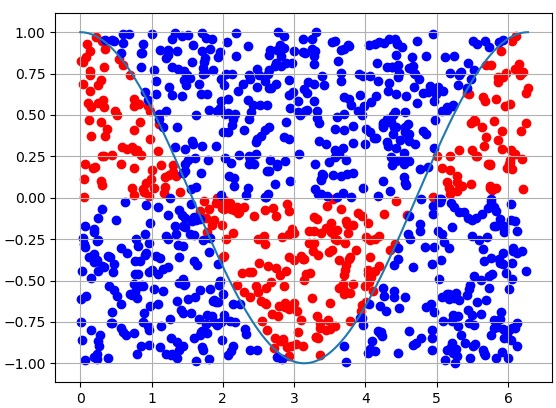
\includegraphics[width=.4\linewidth]{Points}}
        \hspace{.15\linewidth}
        \subfloat[fig2]{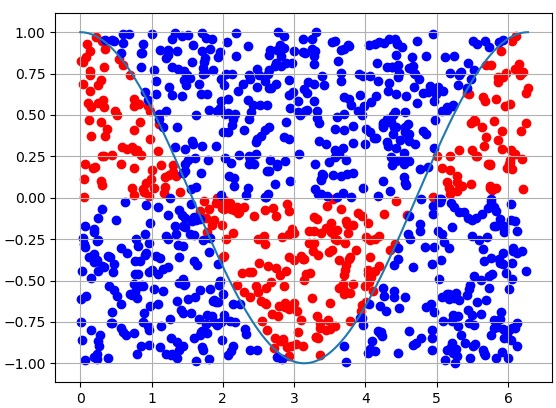
\includegraphics[width=.4\linewidth]{Points}}
        \\
        \subfloat[fig3]{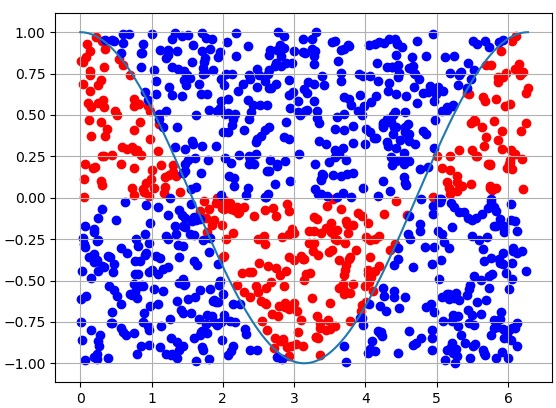
\includegraphics[width=.4\linewidth]{Points}}
        \hspace{.15\linewidth}
        \subfloat[fig4]{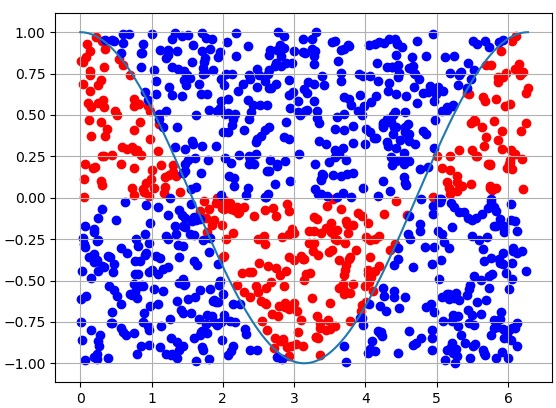
\includegraphics[width=.4\linewidth]{Points}}
        
        \caption{Результат работы программы "Hello, World!"}
    \end{figure}

    \subsection{First section first subsection}

    Hello, here is some text without a meaning.  This text should show what 
    a printed text will look like at this place.  If you read this text, 
    you will get no information.  Really?  Is there no information?  Is there 
    a difference between this text and some nonsense like not at all!  A 
    blind text like this gives you information about the selected font, how 
    the letters are written and an impression of the look.  This text should
    contain all letters of the alphabet and it should be written in of the
    original language.There is no need for special content, but the length of
    words should match the language.

    \begin{itemize}
        
        \item изучить классификацию типов данных и отличительные 
              особенности синтаксических конструкций языка C\# от C++;

        \item изучить базовые типы: Array, String, StringBuilder, а также
              средства стандартного ввода/вывода и возможности форматирования
              вывода;

        \item получить понятие о регулярных выражениях и их применении для поиска,
              замены и разбиения текста на синтаксические лексемы.

    \end{itemize}

    \subsubsection{First section first subsection first subsubsection}

    Hello, here is some text without a meaning.  This text should show what 
    a printed text will look like at this place.  If you read this text, 
    you will get no information.  Really?  Is there no information?  Is there 
    a difference between this text and some nonsense like not at all!  A 
    blind text like this gives you information about the selected font, how 
    the letters are written and an impression of the look.  This text should
    contain all letters of the alphabet and it should be written in of the
    original language.There is no need for special content, but the length of
    words should match the language.

    \begin{enumerate}
        
        \item Проработать примеры программ 1-8, данные в теоретических сведениях.
              Создать на их основе программы. Получить результаты работы программ
              и уметь их объяснить. Внести их в отчет по работе с комментариями.

        \item Найти номер столбца двухмерного массива целых чисел, для которого
              среднеарифметическое его элементов максимально.
              
        \item Создать программу, которая будет вводить строку в переменную String.
              Найти в ней те слова, которые начинаются и заканчиваются одной и той же
              буквой.

        \item Задан текст. Определить, является ли он текстом на английском языке.

    \end{enumerate}

    \subsubsection{First section first subsection second subsubsection}

    Hello, here is some text without a meaning.  This text should show what 
    a printed text will look like at this place.  If you read this text, 
    you will get no information.  Really?  Is there no information?  Is there 
    a difference between this text and some nonsense like not at all!  A 
    blind text like this gives you information about the selected font, how 
    the letters are written and an impression of the look.  This text should
    contain all letters of the alphabet and it should be written in of the
    original language.There is no need for special content, but the length of
    words should match the language.

    \begin{lstlisting}[language={[Sharp]C}]
        namespace ConsoleHello
        { 
            class Program
            {	
                static void Main(string[] args)
                { 
                    Console.WriteLine("Enter your name"); 
                    string name;
                    name = Console.ReadLine();
                    if (name == "") Console.WriteLine("Hello, world!"); 
                    else Console.WriteLine("Hello, " + name + "!");
                }
            }
        }
    \end{lstlisting}

    \subsection{First section second subsection}

    Hello, here is some text without a meaning. This text should show what 
    a printed text will look like at this place. If you read this text, 
    you will get no information.  Really?  Is there no information?  Is there 
    a difference between this text and some nonsense like not at all!  A 
    blind text like this gives you information about the selected font, how 
    the letters are written and an impression of the look.  This text should
    contain all letters of the alphabet and it should be written in of the
    original language.There is no need for special content, but the length of
    words should match the language.

    \begin{equation*}
        \begin{pmatrix}
            1 & 2 & 3 & 4 \\
            5 & 6 & 7 & 8
        \end{pmatrix}
    \end{equation*}

    \begin{figure}[H]
        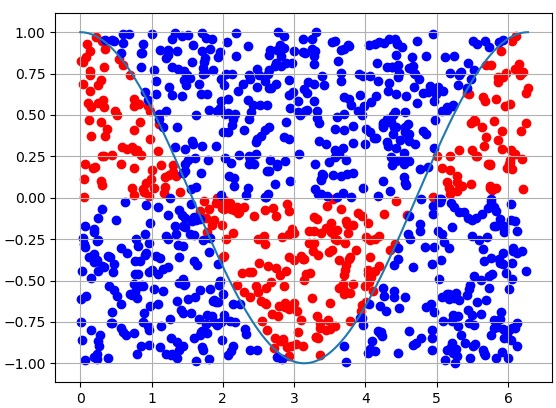
\includegraphics{Points}
        \caption{Какий-та точки в оооооочень длинной подписи к картинке.
            Посмотрим как латек сможет центрировать вторую строку}
    \end{figure}

    \section{Second section}

    Hello, here is some text without a meaning.  This text should show what 
    a printed text will look like at this place.  If you read this text, 
    you will get no information.  Really?  Is there no information?  Is there 
    a difference between this text and some nonsense like not at all!  A 
    blind text like this gives you information about the selected font, how 
    the letters are written and an impression of the look.  This text should
    contain all letters of the alphabet and it should be written in of the
    original language.There is no need for special content, but the length of
    words should match the language.

    \begin{table}[H]
            
        \caption{Какий-та буквы}
        \noindent\begin{tabular}{|c|c|c|c|c|c|c|c|}
            \hline
            cell & cell & cell & cell & cell & cell & cell & cell \\
            cell & cell & cell & cell & cell & cell & cell & cell \\
            cell & cell & cell & cell & cell & cell & cell & cell \\
            \hline
            
        \end{tabular}

    \end{table}

    \subsection{Second section first subsection}

    Hello, here is some text without a meaning.  This text should show what 
    a printed text will look like at this place.  If you read this text, 
    you will get no information.  Really?  Is there no information?  Is there 
    a difference between this text and some nonsense like not at all!  A 
    blind text like this gives you information about the selected font, how 
    the letters are written and an impression of the look.  This text should
    contain all letters of the alphabet and it should be written in of the
    original language.There is no need for special content, but the length of
    words should match the language.

    \begin{itemize}
        \item First item. ello, here is some text without a meaning.  This text should show what 
              a printed text will look like at this place.  If you read this text, 
              you will get no information.  Really?  Is there no information?  Is there 
              a difference between this text and some nonsense like not at all!
        \item First item. ello, here is some text without a meaning.  This text should show what 
               printed text will look like at this place.  If you read this text, 
              you will get no information.  Really?  Is there no information?  Is there 
              a difference between this text and some nonsense like not at all!
        \begin{itemize}
            \item First item first subitem. Hello, here is some text without a meaning.  This text should show what 
                  a printed text will look like at this place.  If you read this text, 
                  you will get no information.  Really?  Is there no information?  Is there 
                  a difference between this text and some nonsense like not at all!
            \item First item second subitem            
        \end{itemize}
    \end{itemize}

\end{document}